% define residuals
% alignment levels

The alignment procedure uses track-based algorithm that updates the locations of detector elements in order to minimize the set of track-hit \emph{residuals}.
These residuals are defined as the distance between the fitted track position in a given detector element to the position of the hit recorded by the same element.
Tracks in ATLAS are parameterized as five-dimensional vectors~\cite{2006.atlas-tracking-model}:%follow helical trajectories and are parameterized as five-dimensional vectors~\cite{2006.atlas-tracking-model}:
\begin{equation}
  \vec{\tau} = (d_0,z_0,\phi_0,\theta,q/p)
\end{equation}
where $d_0$ and $z_0$ are the transverse and longitudinal impact parameters with respect to the origin, respectively, $\phi_0$ is the azimuthal angle of the track at the point of closest approach to the origin, $\theta$ is the polar angle, and $q/p$ is the charge of the track divided by its momentum.
The residual for the $i^{\textrm{th}}$ hit of a given track can then be written in terms of the track parameters $\vec{\tau}$ and the alignment parameters $\vec{a}$ that describe the hit location~\cite{2005.global-chi2-alignment}:
\begin{equation}
  r_i(\vec{\tau},\vec{a}) = (\vec{m}_i - \vec{e}_i (\vec{\tau},\vec{a}))\cdot\hat{k}
\end{equation}
where $\vec{e}_i$ is the intersection point of the extrapolated track with the sensor, $\vec{m}_i$ is the position of the associated hit within the sensor, and $\hat{k}$ is the unit vector defining the direction of the measurement within the sensor.
$\vec{r}$ is then the vector of residuals for the given track.
The effect of a misaligned detector element on the track reconstruction and the resulting track-hit residuals is shown in Figure~\ref{fig:alignment_effects_misalign}. \TODO{ there has to be a better way to introduce this figure}

\begin{figure}[htbp]
  \centering
  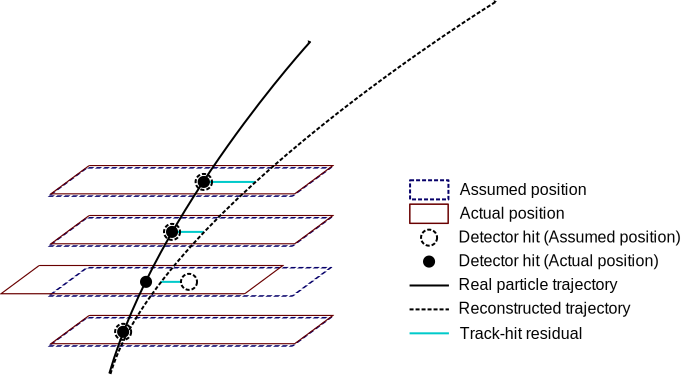
\includegraphics[width=.8\textwidth]{figs/alignment/misalignment}
  \caption{Graphical representation of the effect of a misaligned detector element.  The reconstructed particle track (dashed arrow) differs from the actual trajectory of the particle (solid arrow) due to the shift in one of the detector elements.  The cyan lines represent the track-to-hit residuals.}
  \label{fig:alignment_effects_misalign}
\end{figure}

% the alignment constants are those that minimize the track-hit residuals
A $\chi^2$ function can be built from the residuals of all collected tracks:
\begin{equation}
  \chi^2 = \sum\limits_{\textrm{tracks}}\vec{r}^{T}V^{-1}\vec{r}
  \label{eq:alignment_chi2}
\end{equation}
where $V$ is the covariance matrix of the hit measurements.
The $\chi^2$ function is then minimized with respect to the alignment parameters $\vec{a}$, which contain all degrees of freedom being aligned.
The minimzation condition with respect to $\vec{a}$ is:
\begin{equation}
  \frac{d\chi^2}{d\vec{a}} = 0 ~~ \rightarrow ~~ 2\sum\limits_{\textrm{tracks}}\bigg(\deriv{\vec{r}}{\vec{a}}\bigg)^{T}V^{-1}\vec{r} = 0
  \label{eq:alignment_chi2_min_condition}
\end{equation}
This equation can be difficult to solve exactly, so the residual is rewritten as a first order Taylor expansion:
\begin{equation}
  %\vec{r} = \vec{r}_0+\frac{\partial\vec{r}}{\partial\vec{\tau}}\delta\vec{\tau}+\frac{\partial\vec{r}}{\partial\vec{a}}\delta\vec{a}
  \vec{r} = \vec{r}_0+\deriv{\vec{r}}{\vec{a}}\delta\vec{a}
  \label{eq:alignment_residual_taylor}
\end{equation}
where $\vec{r}_0$ is dependent on an initial set of track and alignment parameters $\vec{\tau}_0$ and $\vec{a}_0$, respectively; the track parameter dependence has also been folded into the total derivative $\deriv{\vec{r}}{\vec{a}}$.
Equation~\ref{eq:alignment_residual_taylor} can then be inserted into the minimization condition from Equation~\ref{eq:alignment_chi2_min_condition} to give:
\begin{equation}
  \Bigg[ \sum\limits_{\textrm{tracks}}\bigg(\deriv{\vec{r}}{\vec{a}}\bigg)^{T}V^{-1}\deriv{\vec{r}}{\vec{a}} \Bigg]\delta\vec{a} + \sum\limits_{\textrm{tracks}}\bigg(\deriv{\vec{r}}{\vec{a}}\bigg)^{T}V^{-1}\vec{r}_0 = 0
  \label{eq:alignment_chi2_min_taylor}
\end{equation}
From this equation, the alignment matrix $\mathcal{M}_a$ and alignment vector $\vec{\nu}_a$ can be defined:
\begin{equation}
  \mathcal{M}_a = \sum\limits_{\textrm{tracks}}\bigg(\deriv{\vec{r}}{\vec{a}}\bigg)^{T}V^{-1}\deriv{\vec{r}}{\vec{a}}
  \label{eq:alignment_matrix}
\end{equation}
\begin{equation}
  \vec{\nu}_a = \sum\limits_{\textrm{tracks}}\bigg(\deriv{\vec{r}}{\vec{a}}\bigg)^{T}V^{-1}\vec{r}_0
  \label{eq:alignment_vector}
\end{equation}
Finally, the alignment corrections $\delta\vec{a}$ can be solved for by inverting the alignment matrix:
\begin{equation}
  \delta\vec{a} = -\mathcal{M}_a^{-1}\vec{\nu}_a
  \label{eq:alignment_corrections}
\end{equation}
%The \emph{alignment constants} are the values of $\vec{a}$ that minimize the track-hit residuals.
which is a linear system of equations with a number of equations equal to the number of alignment degrees of freedom.


\TODO{In practice, the alignment algorithm is iterative . . .}
\TODO{make figure showing iterative procedure as in PoS}

\subsection{Alignment levels}\label{align:levels}
